\documentclass[blue]{beamer}
\usetheme{Warsaw}
\setbeamertemplate{navigation
symbols}{\insertframenumber/\inserttotalframenumber}
\usepackage[francais]{babel}
\usepackage[utf8]{inputenc}
\usepackage[T1]{fontenc}
\usepackage{color}
\usepackage{listings}
\usepackage{geometry}
\usepackage{graphicx}

\definecolor{rltgrey}{rgb}{0.9,0.9,0.9}
\definecolor{rltblue}{rgb}{0.5,0.7,0.9}
%\addtobeamertemplate{footline}{\insertframenumber/\inserttotalframenumber}
\lstset{
language=SQL,                   % choose the language of the code
basicstyle=\ttfamily,           % the size of the fonts that are used for the code
numbers=left,              % where to put the line-numbers numberstyle=\footnotesize,      % the size of the fonts that are used for the line-numbers
stepnumber=0,                   % the step between two line-numbers. If it's1each line will be numbered 
numbersep=5pt,                  % how far the line-numbers are from the code
backgroundcolor=\color{rltblue},% choose the background color.
showspaces=false,               % show spaces adding particular underscores 
showstringspaces=false,         % underline spaces within strings
showtabs=false,                 % show tabs within strings adding particular underscores
frame=single,                   % adds a frame around the code
tabsize=1,                      % sets default tabsize to 2 spaces
captionpos=r,                   % sets the caption-position to bottom
breaklines=true,                % sets automatic line breaking
breakatwhitespace=false,        % sets if automatic breaks should only happen at whitespace
title=\lstname,                 % show the filename of files included with \lstinputlisting;also try caption instead of title
escapeinside={\%*}{*)},         % if you want to add a comment within your code
morekeywords={AND,ASC,avg,CHECK,COMMIT,SAVEPOINT,count,DECODE,BEGIN,DESC,DISTINCT,GROUP,IN,LIKE,NUMBER,ROLLBACK,SUBSTR,sum,VARCHAR2}        
}

\title[Système de fichiers distribué]{Système de fichiers distribué : comparaison de GlusterFS, MooseFS et Ceph avec déploiement sur la grille de calcul Grid’5000.}
\author{\it JF. Garcia, F. Lévigne, \\M. Douheret, V. Claudel}
\date{\today}
\begin{document}

%%%%%%%%%%%%%%%%%%%%%%%%%%%%%%%%%%%%%%%%%%%%%%%%%%%%%%%%%%%%%%%%%%%%%%%%%%%%%%%%%%%%%%%%%%%%%%%%
%\begin{frame}
\titlepage
%\end{frame}
%%%%%%%%%%%%%%%%%%%%%%%%%%%%%%%%%%%%%%%%%%%%%%%%%%%%%%%%%%%%%%%%%%%%%%%%%%%%%%%%%%%%%%%%%%%%%%%%
\begin{frame}{Table des Matières}
\begin{columns}[t]
\begin{column}{5cm}
\tableofcontents[sections={1-4}, hideothersubsections]
\end{column}
\begin{column}{5cm}
\tableofcontents[sections={5-8},hideothersubsections]
\end{column}
\end{columns}
%\tableofcontents[hideothersubsection]
%\tableofcontents[subsectionstyle=hide]
\end{frame}
%%%%%%%%%%%%%%%%%%%%%%%%%%%%%%%%%%%%%%%%%%%%%%%%%%%%%%%%%%%%%%%%%%%%%%%%%%%%%%%%%%%%%%%%%%%%%%%%
%%%%%%%%%%%%%%%%%%%%%%%%%%%%%%%%%%%%%%%%%%%%%%%%%%%%%%%%%%%%%%%%%%%%%%%%%%%%%%%%%%%%%%%%%%%%%%%%
%%%%%%%%%%%%%%%%%%%%%%%%%%%%%%%%%%%%%%%%%%%%%%%%%%%%%%%%%%%%%%%%%%%%%%%%%%%%%%%%%%%%%%%%%%%%%%%%
\section{Introduction}
	\subsection{Présentation du sujet}
	\begin{frame}
		\frametitle{Présentation du sujet}
		Comparaison de systèmes de fichiers distribué :
		\begin{itemize}
			\item Système de fichier (FS) : façon de stocker, organiser des informations dans un fichier
			\item Système de fichiers distribué :
			\begin{itemize}
				\item Éclaté sur plusieurs serveurs % éclaté ? Un meilleur mot ?
				\item Disponible depuis plusieurs clients
			\end{itemize}
		\end{itemize}
	\end{frame}

	\subsection{Le Grid'5000}
	\begin{frame}
		\frametitle{Le Grid'5000}
		\begin{itemize}
			\item Infrastructure distribué dédiée à la recherche
			\item 11 sites, dont 9 en France
			\begin{figure}
				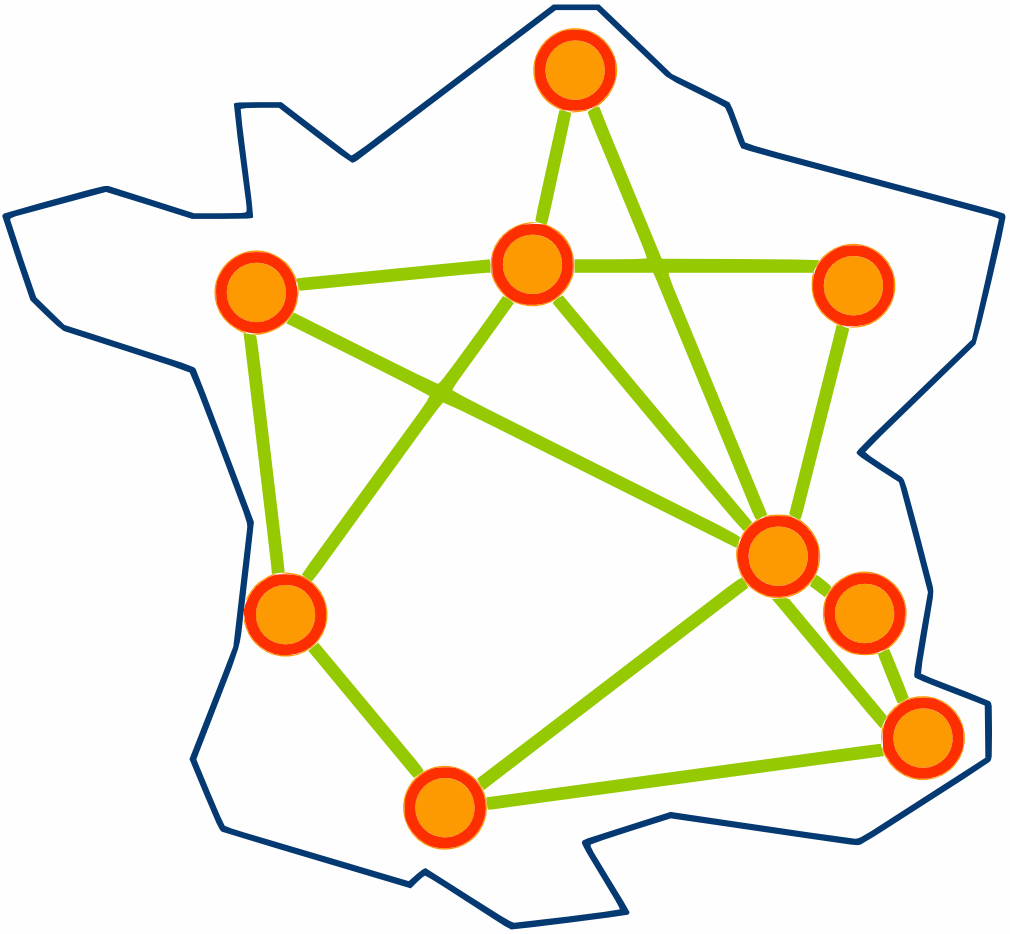
\includegraphics[width=0.3\linewidth]{../images/Site_map.png}
				\caption{Les sites français du Grid'5000}
			\end{figure}
		\end{itemize}
	\end{frame}

	\begin{frame}
		\frametitle{Travailler sur le Grid'5000}
		\begin{itemize}
			\item Connexion au \og frontend\fg~ par SSH
			\item Réservation de nœuds, pour un certain temps
			\item Déploiement d'image (OS)
		\end{itemize}

		\begin{block}{Astuce :}
			Possibilité d'effectuer une réservation à l'avance, suivit par l'exécution d'un script
		\end{block}
	\end{frame}

\section{NFS}
  \subsection{Présentation de NFS}
\begin{frame}
  \frametitle{Présentation de NFS}
  \begin{itemize}
    \item Network File System
    \item Développé par Sun Microsystem
    \item Partager des données par le réseau
    \item Méthode standard de partage entre machines Unix
  \end{itemize}
\end{frame}

\subsection{Aspect technique}
\begin{frame}
  \frametitle{Aspect technique}
  \begin{itemize}
    \item NFS et le protocole non connecté UDP
    \item Depuis la version 3, possibilité d'utiliser TCP
    \item NFSv1 et v2 définies dans la RFC 1094
    \item NFSv3 définie dans la RFC 1813
    \item NFSv4 définie dans la RFC 3010 et dans la RFC 3530 :
    \begin{itemize}
      \item meilleur gestion de la sécurité
      \item meilleur gestion de la montée en charge
      \item système de maintenance simplifié
      \item support des protocoles TCP (par défaut) et RDMA
  \end{itemize}
  \end{itemize}
\end{frame}

\subsection{Mise en place}
	\begin{frame}
		\frametitle{Mise en place}
		\begin{itemize}
			\item Licence GPLv3
			\item Capacité pouvant atteindre plusieurs petabytes (1000 To)
			\item Structure simple, deux éléments logiciels : serveur et client
			\item Supporte plusieurs protocoles de communications (TCP/IP, InfiniBand)
		\end{itemize}
	\end{frame}
	
\section{GlusterFS}
	\subsection{Présentation de GlusterFS}
	\begin{frame}
		\frametitle{Présentation de GlusterFS}
		\begin{itemize}
			\item Licence GPLv3
			\item Se base sur FUSE (Filesystem in UserSpacE)
			\item Capacité pouvant atteindre plusieurs petabytes (1000 To)
			\item Structure simple, deux éléments logiciels : serveur et client
			\item Supporte plusieurs protocoles de communications (TCP/IP, InfiniBand)
		\end{itemize}
	\end{frame}
	
	\subsection{Mise en place}
	\begin{frame}
		\frametitle{Mise en place}
		\begin{itemize}
			\item Un serveur maitre : paquet glusterfs-server
			\item x serveurs \og normaux\fg
			\item x clients : glusterfs-client
		\end{itemize}

		\begin{block}{Note :}
			Les serveurs doivent avoir un répertoire dédié au partage
		\end{block}
	\end{frame}

	\begin{frame}
		\frametitle{Mise en place (2)}
			\begin{itemize}
				\item A partir du serveur maitre :
				\begin{itemize}
					\item Génération des fichiers de configurations (commande prévue)
					\item Envoie de fichiers aux serveurs, et aux clients
				\end{itemize}
				\item Démarrage des serveurs
				\item Montage du volume par les clients
			\end{itemize}
	\end{frame}

	\subsection{Difficultés rencontrées}
	\begin{frame}
		\frametitle{Difficultés rencontrées}
			\begin{itemize}
				\item Droit d'écriture des clients
				\item Utilisation d'InfiniBand
				\item Script de déploiement : automatisation totale
			\end{itemize}
		\end{frame}


\section{MooseFS}
\begin{frame}

\end{frame}

\section{Ceph}
        \subsection{Présentation}
        \begin{frame}
                \frametitle{Présentation de Ceph}
		\begin{itemize}
			\item Licence LGPL
			\item créer par Sage Weill en 2007
			\item destiné au très grands clusters
			\item but principal : 
                              \begin{itemize}
                                      \item compatible POSIX
                                      \item complétement distribué sans point de défaillance
                              \end{itemize}
		\end{itemize}
        \end{frame}
        
        \begin{frame}
                \frametitle{Caractéristique}
                \begin{itemize}
                        \item caractéristique de Ceph :
                        \begin{itemize}
                                \item robustesse
                                \item évolutivité transparente
                        \end{itemize}
                \end{itemize}
        \end{frame}

        \begin{frame}
                \frametitle{Fonctionnement}
                \begin{itemize}
                        \item trois types distincts de démons :
                        \begin{itemize}
                                \item moniteur de cluster
                                \item serveurs de métadonnées
                                \item serveurs de données
                        \end{itemize}
                \end{itemize}
        \end{frame}

        \begin{frame}
                \frametitle{Moniteur}
                \begin{itemize}
                        \item 
                \end{itemize}
        \end{frame}

\section{Comparaison}
\begin{frame}

\end{frame}

\section{Conclusion}
\begin{frame}

\end{frame}

\end{document}
